\section{Baseline results of the reduced-order model}
\label{sec:baseline}

All values in this section are computed by the program \texttt{code/hff\_model.py} from the inputs of
Tables~\ref{tab:geometry} and~\ref{tab:props} and the relations of Section~\ref{sec:reduced};
Table~\ref{tab:baseline} collects them. Quantities that depend on the solid properties scale with
the datasheet values, which are not frozen (A3).

\begin{table}[t]
\centering\small
\caption{Reduced-order baseline at the design point of Table~\ref{tab:geometry}. The deflection and
passage height are given for the self-consistent state (sc) and, as an upper bound, for the
frozen-force state (ff).}
\label{tab:baseline}
\begin{tabular}{@{}p{4.4cm}p{4.6cm}p{4.9cm}@{}}
\toprule
Quantity & Expression & Value \\
\midrule
Reynolds, P\'eclet numbers & $2\rho UH_0/\mu$; $\mathrm{Re}\,\mathrm{Pr}$ & $\NumRe$; $\NumPe$ (Pr $=\NumPr$) \\
Rigid-slit pressure drop & $12\mu UL/H_0^2$ \eqref{eq:dp} & \SI{\NumDp}{\pascal}; wall shear \SI{\NumTauW}{\pascal} \\
Through-wall temperature drop & $\Delta T_t=\qpp d/k_s$ & \SI{\NumDTt}{\kelvin} \\
Bulk rise; interface excess & $\Delta T_b$; $\qpp/h$ with $h=\NumHrigid\,\si{\watt\per\square\metre\per\kelvin}$ & \SI{\NumDTb}{\kelvin}; \SI{\NumQoverH}{\kelvin} \\
Mean wall temperature rise & $\bar\theta=\Delta T_t/2+\qpp/h+\Delta T_b/2$ & \SI{\NumThetaBar}{\kelvin} \\
Free thermal curvature & $(1+\nu)\alpha\qpp/k_s$ \eqref{eq:kappa} & \SI{\NumKappa}{\per\metre} \\
Linear bow & $\kth L^2/8$ \eqref{eq:wlin} & $\NumWlin$~m $=\NumWlinH\,H_0$ \\
Membrane force; Euler load & $N_c$ \eqref{eq:ntheta}; $\ncr=\pi^2D_s/L^2$ & $\NumNtheta$; $\NumNcr$ N\,m$^{-1}$; $N_c/\ncr=\NumNratio$ \\
Critical rise; buckling margin & $\bar T_{\mathrm{cr}}$; $M_b$ \eqref{eq:tcr} & \SI{\NumTcr}{\kelvin}; $\NumMb$ \\
Beam--column parameter & $\mu L=L\sqrt{N_c/D_s}$ & $\NumMuL$ \\
Bow, frozen force (ff) & \eqref{eq:wbc} & $\NumWfrozen$~m $=\NumWfrozenH\,H_0$ \\
Bow, self-consistent (sc) & \eqref{eq:wbc}, \eqref{eq:nupdate} & $\NumWsc$~m $=\NumWscH\,H_0$ \\
Mid-span passage height $H_0+\wmax$ & derived & $\NumHmidSc\,H_0$ (sc); $\NumHmidFrozen\,H_0$ $=$ \SI{\NumHmidMm}{\milli\metre} (ff) \\
Slope, strains (ff) & $\max|w^\prime|$; $\tfrac12\langle w^{\prime2}\rangle$; bending fibre strain & $\NumSlope$; $\NumArcStrain$; $\NumFibreStrain$ \\
Stresses (ff) & bending; membrane; sum & \SI{\NumSigBend}{\mega\pascal}; \SI{\NumSigMemb}{\mega\pascal}; \SI{\NumSigMax}{\mega\pascal} $=\NumSigFrac\,\sigma_y$ \\
Gauge pressure on the strip & $p(0)$; $p(L)$; $\bar p$ & \SI{\NumPentry}{\pascal}; \SI{\NumPexit}{\pascal}; \SI{\NumPbar}{\pascal} \\
Hydraulic deflection & $5\bar pL^4/(384D_s)$ & $\NumWp$~m (zero force); $\NumWpBC$~m (with $N_c$) \\
Thermal-to-hydraulic ratio & $\Gamma_p^{\mathrm{lin}}$; $\Gamma_p^{N_c}$ \eqref{eq:gammap} & $\NumGammaLinRound$; $\NumGammaBCRound$ \\
Buoyancy, dissipation & $\mathrm{Ri}$; $\mathrm{Br}$ & $\NumRi$; $\NumBr$ \\
\bottomrule
\end{tabular}
\end{table}

\subsection{Deformation of the passage}
\label{sec:deform}
The strip bows away from the channel by $\wmax=\NumWsc$~m, which is $\NumWscH\,H_0$, in the
self-consistent state; the frozen-force upper bound is $\NumWfrozenH\,H_0$
(Figure~\ref{fig:bowing}a). The passage height at mid-span is $H=H_0+\wmax=\NumHmidSc\,H_0$
(sc) or $\NumHmidFrozen\,H_0$ (ff), that is \SI{\NumHmidMm}{\milli\metre} against the undeformed
\SI{0.50}{\milli\metre}. This is a \emph{derived beam-model passage height}, not a prescribed
clearance: it is the sum of the design height $H_0$ and the computed deflection, and nothing in the
model constrains it from above (assumption A9). A two-dimensional finite-element solution of the restrained wall (Section~\ref{sec:q8nl}) gives
$\NLwFEH\,H_0$, $\NLoverScPct\,\%$ above the self-consistent value.
The beam--column amplification over the linear bow
is $\NumAmpFrozen$, consistent at leading order with the Euler factor $1/(1-N_c/\ncr)=\NumAmpEuler$.
The strains and the slope are small ($\max|w^\prime|=\NumSlope$, bending fibre strain
$\NumFibreStrain$), which supports the small-strain, moderate-rotation level of A4.

\begin{figure}[t]
\centering
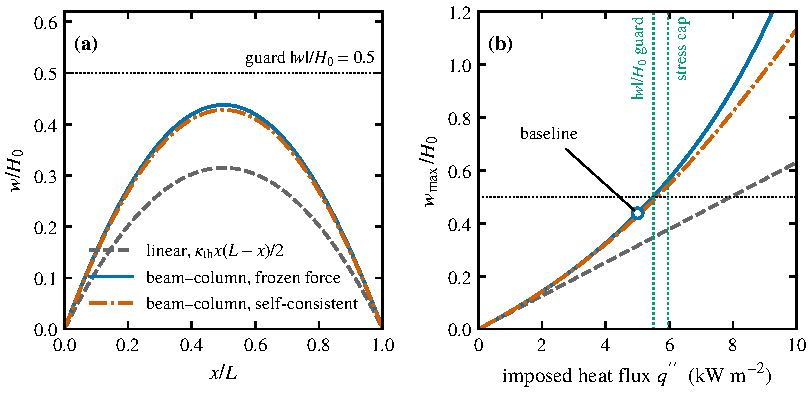
\includegraphics[width=\textwidth]{figures/fig2_bowing.pdf}
\caption{Bowing of the strip (positive away from the channel). (a) Deflection profile at the
baseline: linear estimate \eqref{eq:wlin}, frozen-force beam--column \eqref{eq:wbc} and
self-consistent beam--column \eqref{eq:wbc}--\eqref{eq:nupdate}. (b) Mid-span deflection against the
imposed flux; vertical dotted lines mark the fluxes at which guards G1 ($|w|/H_0=0.5$) and G2
(stress cap) are reached. The marker is the baseline.}
\label{fig:bowing}
\end{figure}

\subsection{Guards and heat-flux ceilings}
\label{sec:ceilings}
The baseline lies inside all five guards of Section~\ref{sec:guards}: $\wmax/H_0=\NumWfrozenH$ (ff)
against 0.5; $\sigma_{\max}=\NumSigFrac\,\sigma_y$ against 0.2; $M_b=\NumMb$ against 2;
$\Gamma_p=\NumGammaLinRound$ against 5; $\mathrm{Re}_{D_h}=\NumRe$, $\mathrm{Br}=\NumBr$ and
$\mathrm{Ri}=\NumRi$. All but the last are exceeded in the order deformation, stress, buckling as
$\qpp$ increases, because $\kth$ and $\bar\theta$ both scale with $\qpp$. In the frozen-force state G1
is reached at $\qpp=\SI{\NumQw}{\kilo\watt\per\square\metre}$ ($N_c/\ncr=\NumRatioW$), G2 at
\SI{\NumQs}{\kilo\watt\per\square\metre} ($\wmax/H_0=\NumWHs$), and the buckling margin $M_b=2$ at
\SI{\NumQb}{\kilo\watt\per\square\metre}, where $\wmax/H_0=\NumWHb$ would long since be
unacceptable. The binding constraints are therefore deformation and stress, with buckling the outer
ceiling, and the baseline flux is already \SI{9}{\percent} below the first of them.

Buoyancy and viscous dissipation do not enter the baseline: $\mathrm{Ri}=\NumRi$ and $\mathrm{Br}=\NumBr$.
Stratification can destabilise horizontal flows when it is strong, as studied for a fluid with large
property variations by \citet{draskic2025stability}; that regime is not approached here.

The stress is dominated by the compressive membrane component, \SI{\NumSigMemb}{\mega\pascal}, a
by-product of the axial constraint that also produces the buckling limit; the bending component is
\SI{\NumSigBend}{\mega\pascal}.

\subsection{Role of the wall material}
Because $\kth=(1+\nu)\alpha\qpp/k_s$, the choice of wall material sets the size of the effect. For
typical austenitic stainless steel ($k_s\approx\SI{16}{\watt\per\metre\per\kelvin}$,
$\alpha\approx\SI{1.7e-5}{\per\kelvin}$, $\nu=0.30$) at the same flux and geometry,
$\kth=\NumStainlessKappa$~\si{\per\metre} and $\wmax^{\mathrm{lin}}/H_0=\NumStainlessWH$: about
$\NumPolymerOverStainless$ times smaller than for the polymer, a physically real deformation but
irrelevant to the convective field. The combination of low conductivity and high expansion
coefficient of the polymer class, not any fluid-side property, selects the design space.

\subsection{Indicative consequences for the flow}
\label{sec:indicative}
The deformation is large enough to change the passage substantially, so two flow-side consequences
are estimated. Both are reduced-order and indicative only; the coupled computation is required to
quantify them. \emph{Hydraulic.} With the flow rate per unit depth $UH_0$ fixed and the local height
$H(x)=H_0+w(x)$, the lubrication estimate is
$\Delta p=12\mu UH_0\int_0^L\dd x/H^3$, which is $\NumDpLub$~Pa, a factor $\NumDpLubRatio$ of the
rigid-slit value \eqref{eq:dp}, a drop of about $\NumDpLubDrop$ per cent (Figure~\ref{fig:passage}b).
The lubrication parameter $\mathrm{Re}_{H_0}H_0/L=\NumReHL$ is not small, so the value indicates that the
hydraulic effect is of order one rather than giving its magnitude. \emph{Thermal.} With a
quasi-developed local coefficient $h(x)=\mathrm{Nu}_{H1}k_f/[2H(x)]$ the mean interface excess
$\qpp/h$ rises from \SI{\NumQoverH}{\kelvin} to \SI{\NumExcessDeformed}{\kelvin} (a factor
$\NumExcessRatio$). The thermal entry length is about \SI{\NumLT}{\milli\metre}, so $L/L_T=\NumLoverLT$
and the quasi-developed assumption is not justified; this too is an order-of-magnitude indicator.

\begin{figure}[t]
\centering
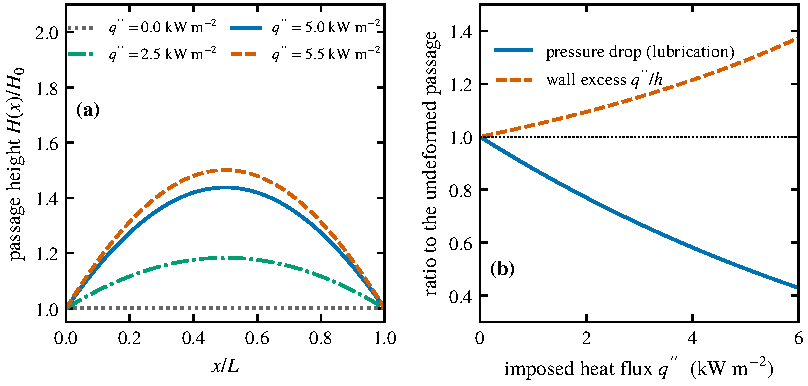
\includegraphics[width=\textwidth]{figures/fig3_passage.pdf}
\caption{Reduced-order consequences of the deformation (indicative). (a) Passage height $H(x)/H_0$
for several imposed fluxes (frozen-force bow). (b) Lubrication estimate of the pressure drop and
quasi-developed estimate of the mean interface excess $\qpp/h$, both relative to the undeformed
passage.}
\label{fig:passage}
\end{figure}

\emph{Feedback onto the deflection.} The larger interface excess raises $\bar\theta$ by about
\SI{\NumFeedbackExtraK}{\kelvin} out of \SI{\NumThetaBar}{\kelvin}, which increases $\wmax$ by only
\NumFeedbackPct\,\%; the hydraulic load changes the deflection by $\NumHydFeedbackPct$\,\% of the
thermal bow ($1/\Gamma_p$). At the baseline the effect of the wall on the flow is therefore large,
whereas the effect of the flow back on the wall is small, because $\kth$ depends on $\qpp$ and on the wall
properties only (equation~\eqref{eq:kappa}) and the thermal loop enters through $\bar\theta$ alone.
Whether the closed loop matters elsewhere in the parameter space is a question for the coupled
computation, not for this reduced-order model.
